\chapter[Pulsar geometry and carousel geometry]{The geometric model}
\label{app: geometry derivations}

\citet{DRxx2001} published a set of equations that map observed emission as a function of time to an image of the beam pattern which circulates around the magnetic axis. Here, time is quantified by a pulse number $k$ and pulse longitude $\phi$, and these are related to polar coordinates co-rotating with the carousel centred on the magnetic axis, thereby producing an image of the pulsar beam with a stationary carousel. One can apply the cartographic transform to a $P_3$-fold by relating the integer $k$ cyclically to the phase in the modulation cycle (i.e. the $y$-axis of the plots in Fig.~\ref{fig: B0031 - observed P3folds}). At a given time radiation is observed which is emitted in a direction which makes an angle $R$ with respect to the magnetic axis (polar angle), and azimuthal angle $\Theta$ in the beam map (in a frame co-rotating with the carousel).

If the circulation period $P_4$ is set to the rotation period of the carousel, then the frame is co-rotating with the beamlets such that their associated azimuthal angles remain constant. For a circular carousel, the transforms can be written as
\begin{equation}
    \label{eq: cartographic transform - R}
    \sin^2\bigg(\frac{R}{2}\bigg) = \sin^2\bigg(  \frac{\Delta\phi}{2} \bigg)\sin(\alpha)\sin(\zeta) + \sin^2\bigg(\frac{\beta}{2} \bigg),
\end{equation}
\begin{equation}
    \label{eq: cartographic transform - Theta}
    \Theta = \theta_\mathrm{trans} + \theta_\mathrm{rot},
\end{equation}
    where
\begin{equation}
    \label{eq: cartographic transform - sin theta_trans}
    \sin(\theta_\mathrm{trans}) = \frac{\sin(\zeta)\sin(\Delta\phi)}{\sin(R)},
\end{equation}
\begin{equation}
    \label{eq: cartographic transform - cos theta_trans}
    \cos(\theta_\mathrm{trans}) = \frac{\cos(\alpha)\cos(R) - \cos(\zeta)}{\sin(\alpha)\sin(R)},
\end{equation}
    and
\begin{equation}
    \label{eq: cartographic transform - theta_rot}
    \theta_\mathrm{rot} =  \mp \bigg(2\pi k + \Delta\phi\bigg)\frac{P_1}{P_4}.
\end{equation}
In these equations, $\Delta\phi = \phi - \phi_\mathrm{fid}$, where $\phi_\mathrm{fid}$ is the pulse longitude corresponding to the fiducial plane, the plane which contains the magnetic and rotation axes. The inclination of the magnetic axis with respect to the rotation axis is $\alpha$, $\beta$ is the impact parameter of the observer's line of sight (LOS) with respect to the magnetic axis, and $\zeta = \alpha + \beta$. The changing orientation of the LOS with respect to the magnetic axis is quantified with $\theta_\mathrm{trans}$ and the rotation of the carousel is quantified with $\theta_\mathrm{rot}$. The period of rotation of the carousel is $P_4$ and $P_1$ is the rotation period of the star. In Eq.~\eqref{eq: cartographic transform - theta_rot}, the $(-)$ applies if $\alpha<90\degr$, whilst the $(+)$ applies if $\alpha>90\degr$\footnote{Wherever a $\pm$ or $\mp$ sign appears in this appendix, care has been taken in its use such that the upper sign will correspond to the $\alpha < 90\degr$ case, and the lower sign to the $\alpha > 90\degr$ case.}.

I extend these equations to deal with the case where the carousel is aliased, and also modified to describe the transformation to and from a $P_3$-fold as well as a simple pulse stack. In order to help the reader understand these extensions, this appendix first gives a full derivation of the transform to reach the form above, before working through the additions required for Chapter.~\ref{chapt: B0031}.









\section{Derivation of the cartographic transform}
\label{app: geometry derivations - cartographic transform}

The geometry of the emission region of a pulsar is shown in Fig.~\ref{fig: geometry derivations - full emission region geometry}. All quantities referred to in the cartographic transforms are labelled. The emission region (yellow circle) surrounds the magnetic axis $\mathbf{B}$ which sits at an inclination angle $\alpha$ to the rotation axis $\mathbf{\Omega}$. The observer's line of sight passes across the emission region with the impact parameter $\beta$, crossing the fiducial plane at a longitude $\phi_\mathrm{fid}$. As the star rotates, the footprint of the LOS moves around $\mathbf{\Omega}$ with respect to the emission beam such that at an arbitrary phase $\phi$ it is at angular distance $R$ from the magnetic axis. These angles are measured with respect to the centre of the star. The angle $\theta_\mathrm{trans}$ shows the azimuthal angle the footprint of the LOS makes with the fiducial plane (so not defined in the carousel frame, unlike $\Theta$) and is defined clockwise about the magnetic axis when viewed from above. In Fig~\ref{fig: geometry derivations - full emission region geometry} the star rotates anticlockwise when viewed from above, such that the emission regions move from left to right as depicted.
\begin{figure}
    \begin{center}
        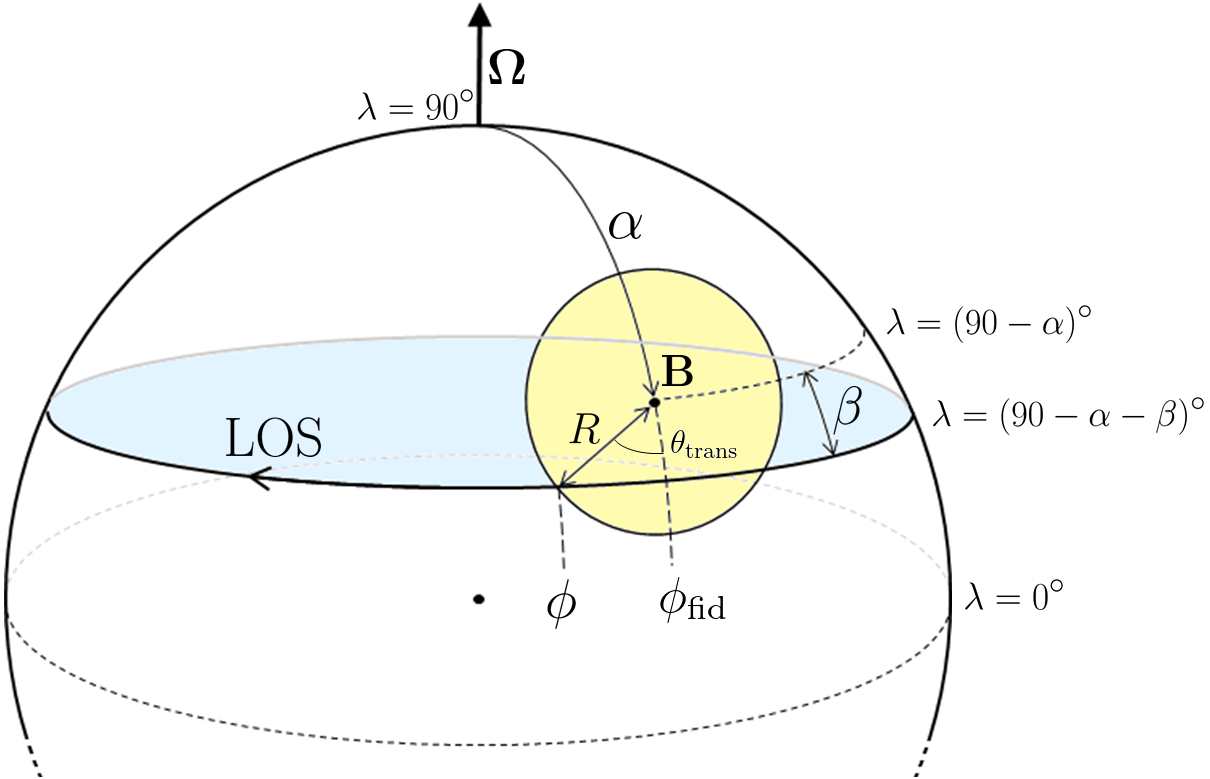
\includegraphics[width=0.8\textwidth]{Figures/geometry_appendix/full_geom}
        \caption[Emission region geometry]{A schematic representation of a circular emission region centred on the magnetic axis $\mathbf{B}$, which is inclined at an angle $\alpha$ to the rotation axis. The observer's line of sight (LOS) passes by the magnetic axis with an impact angle $\beta$. The footprint of the LOS crosses the midpoint of the emission region (the fiducial plane) at a phase $\phi_\mathrm{fid}$, and at a subsequent phase $\phi$ is at an angular distance $R$ from $\mathbf{B}$. The (rotational) latitude of the LOS is $\lambda = (90-\alpha-\beta)\degr$, and the magnetic axis lies at latitude $\lambda = (90-\alpha)\degr$. }
        \label{fig: geometry derivations - full emission region geometry}
    \end{center}
\end{figure}
The rotational equator of the star defines latitude $\lambda = 0\degr$, and the rotational north pole is at $\lambda = +90\degr$. This means that the latitude of the magnetic axis is $\lambda_\mathbf{B} = (90 - \alpha)\degr$, and the LOS delineates a plane (shown in blue in Fig.~\ref{fig: geometry derivations - full emission region geometry}) at a latitude $\lambda_\mathrm{LOS} = (90 - \alpha - \beta)\degr$.


\begin{figure}
    \begin{center}
        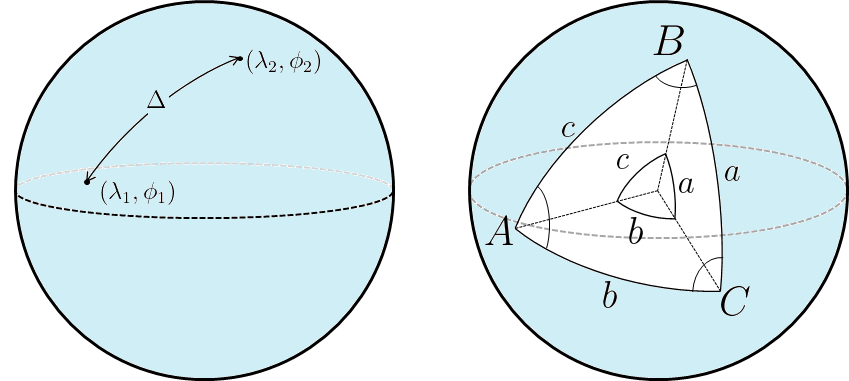
\includegraphics[width=0.75\textwidth]{Figures/geometry_appendix/spherical_geometry}
        \caption[Spherical trigonometry]{(LEFT) The angular distance between two points on a sphere is $\Delta$, and (RIGHT) the angles defining a spherical triangle.}
        \label{fig: geometry derivations - spherical trigonometry}
    \end{center}
\end{figure}
In Fig.~\ref{fig: geometry derivations - spherical trigonometry} a triangle on the surface of a sphere is defined, which is used in the derivation of the cartographic transforms. The left-hand image illustrates the great circle distance $\Delta$ between two points on the surface of a sphere. The two points have coordinates in latitude and longitude of $(\lambda_1, \phi_1)$ and $(\lambda_2, \phi_2)$ respectively. The right-hand side of Fig.~\ref{fig: geometry derivations - spherical trigonometry} shows a spherical triangle formed between three points by great circle arcs. the angles $A$, $B$, and $C$ are the angles between the sides of the triangle, whilst $a$, $b$, and $c$ are the angles subtended by the great circle arcs at the centre of the sphere.

The first relevant relation gives the great circle distance between two points on the sphere. The quantity $\sin^2(\Delta/2)$ is known as the \textit{haversine} of $\Delta$, and the \textit{haversine formula} for the angular distance between two points $(\lambda_1, \phi_1)$ and $(\lambda_2, \phi_2)$ is
\begin{equation}
    \label{eq: geometry derivations - haversine}
	\sin^2\bigg(\frac{\Delta}{2}\bigg) = \sin^2\bigg(\frac{\phi_2 - \phi_1}{2}\bigg) \cos(\lambda_1)\cos(\lambda_2) + \sin^2\bigg(\frac{\lambda_2 - \lambda_1}{2}\bigg),
\end{equation}
where latitude is denoted by $\lambda$, and longitude is $\phi$ (in radians). The second and third relations required for derivation of the cartographic transforms are the spherical sine and cosine rules (with reference to the right-hand panel of Fig.~\ref{fig: geometry derivations - spherical trigonometry}),
\begin{equation}
    \label{eq: geometry derivations - spherical sine}
    \frac{\sin A}{\sin a} = \frac{\sin B}{\sin b} = \frac{\sin C}{\sin c},
\end{equation}
\begin{equation}
    \label{eq: geometry derivations - spherical cosine}
    \cos a = \cos b \cos c + \sin b \sin c \cos A. 
\end{equation}



















\subsection{Derivation of the radial distance, \texorpdfstring{$R$}{\textit{R}}}
\label{app: geometry derivations - cartographic transforms - derivation of R}

Figure \ref{fig: geometry derivations - theta trans triangle} shows a closer view of the pulsar geometry shown in Fig.~\ref{fig: geometry derivations - full emission region geometry}, focusing on the spherical triangle defined between the magnetic axis $\mathbf{B}$, the rotation axis $\mathbf{\Omega}$, and the `visible point' on the observer's line of sight (LOS). The angular distance between a given point on the LOS and the magnetic axis is $R$. The magnetic axis is located at latitude $\lambda_\mathbf{B} = (90-\alpha)\degr$ and its longitude is the origin, $\phi_\mathrm{fid}$. An arbitrary point on the LOS has corresponding coordinates $\lambda_\mathrm{LOS} = (90 - \alpha - \beta)$ and longitude $\phi$. Substituting these values into the haversine formula (Eq.~\eqref{eq: geometry derivations - haversine}),
\begin{equation}
    \sin^2\bigg(\frac{R}{2}\bigg) = \sin^2\bigg(\frac{\phi - \phi_\mathrm{fid}}{2}\bigg) \sin(\alpha)\sin(\alpha + \beta) + \sin^2\bigg(\frac{\beta}{2}\bigg) \label{eq: geometry derivations - derived R}.
\end{equation}
With the substitutions $\zeta = \alpha + \beta$ and $\Delta\phi = \phi - \phi_\mathrm{fid}$, this is the first of the transform equations (Eq.~\eqref{eq: cartographic transform - R}).













\subsection{Derivation of the azimuthal angle, \texorpdfstring{$\Theta$}{Theta}}
\label{app: geometry derivations - cartographic transforms - derivation of Theta}

\subsubsection{Angle due to the rotation of the star}
\label{app: geometry derivations - cartographic transforms - derivation of Theta - theta trans}

The azimuthal offset $\Theta$ of a point on the polar map in the co-rotating frame of the carousel from an arbitrary meridian has two components, $\theta_\mathrm{trans}$ and $\theta_\mathrm{rot}$. $\theta_\mathrm{trans}$ is the component due to the movement of the footprint of the LOS past the magnetic axis, and $\theta_\mathrm{rot}$ is due to the circulation of the carousel itself. The first of these, $\theta_\mathrm{trans}$, can be derived by considering a spherical triangle formed between the rotation axis $\mathbf{\Omega}$, the magnetic axis $\mathbf{B}$, and a point on the LOS at an angular distance $R$ from the magnetic axis in accordance with Eq.~\eqref{eq: geometry derivations - derived R}, as illustrated in Fig.~\ref{fig: geometry derivations - theta trans triangle}.
\begin{figure}
    \begin{center}
        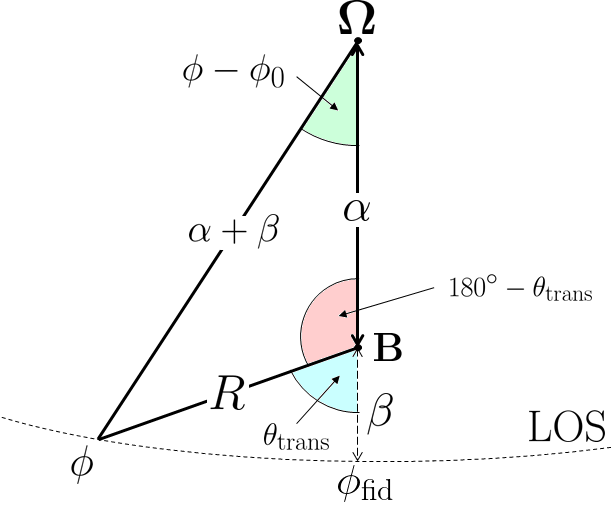
\includegraphics[width=0.5\textwidth]{Figures/geometry_appendix/theta_trans}
        \caption[The spherical triangle that describes pulsar geometry]{The spherical triangle formed between the magnetic ($\mathbf{B}$) and rotation ($\mathbf{\Omega}$) axes and a point on the line of sight (LOS). The point on the line of sight is offset from the magnetic axis by an angular distance $R$, and is offset in longitude by $\phi - \phi_\mathrm{fid}$. The azimuthal offset between $R$ and the fiducial plane at $\phi_\mathrm{fid}$ is $\theta_\mathrm{trans}$.}
        \label{fig: geometry derivations - theta trans triangle}
    \end{center}
\end{figure}

From Fig.~\ref{fig: geometry derivations - theta trans triangle} and the spherical sine rule (Eq.~\eqref{eq: geometry derivations - spherical sine}),
\begin{equation}
    \label{eq: sthetatrans1}
	\frac{\sin(\phi-\phi_\mathrm{fid})}{\sin R} = \frac{\sin (180\degr - \theta_\mathrm{trans})}{\sin (\alpha + \beta)}.
\end{equation}
Or,
\begin{equation}
    \label{eq: sthetatrans2}
	\sin\theta_\mathrm{trans} = \frac{\sin(\alpha + \beta) \sin(\phi-\phi_\mathrm{fid})}{\sin R};
\end{equation}
which is the sine component of $\theta_\mathrm{trans}$ as given in Eq.~\eqref{eq: cartographic transform - sin theta_trans}. The cosine component arises from the spherical cosine rule (Eq.~\eqref{eq: geometry derivations - spherical cosine}):
\begin{equation}
    \label{eq: cthetatrans1}
    \cos (\alpha + \beta) = \cos \alpha \cos R + \sin \alpha \sin R \cos (180\degr - \theta_\mathrm{trans}),
\end{equation}
which can be rearranged as
\begin{equation}
    \label{eq: cthetatrans2}
    \cos(\theta_\mathrm{trans}) = \frac{\cos(\alpha)\cos(R) - \cos(\zeta)}{\sin(\alpha)\sin(R)},
\end{equation}
and reproduces Eq.~\eqref{eq: cartographic transform - cos theta_trans}. Both the sine and cosine components of $\theta_\mathrm{trans}$ are needed to find a solution for $\theta_\mathrm{trans}$ that lies in the right quadrant.







\subsubsection{Angle due to the circulation of the carousel}
\label{app: geometry derivations - cartographic transforms - derivation of Theta - theta rot}

The second angle $\theta_\mathrm{rot}$ is simply a phase shift in $\theta_\mathrm{trans}$ in order to go to a frame co-rotating with the carousel. It depends on the carousel rotation period, $P_4$, and time. Time is quantified the pulse number $k$ and the rotational phase $\phi$. Thus,
\begin{equation}
    \label{eq: thetarot}
	\theta_\mathrm{rot} = \mp \frac{2\pi P_1}{P4}\bigg( k + \frac{\phi - \phi_\mathrm{fid}}{2\pi}\bigg).
\end{equation}

The sign in Eq.~\eqref{eq: thetarot} defines the direction of rotation of the carousel. For a carousel which circulates in the same direction as the pulsar rotates (but lagging co-rotation as predicted by \citealt{RSxx1975}), the $(-)$ sign applies for a carousel in the northern rotational hemisphere (i.e. if $\alpha < 90\degr$) while the $(+)$ sign applies for a carousel in the southern hemisphere ($\alpha > 90\degr$). This is illustrated in Fig.~\ref{fig: geometry derivations - carousel direction}.
\begin{figure}
    \begin{center}
        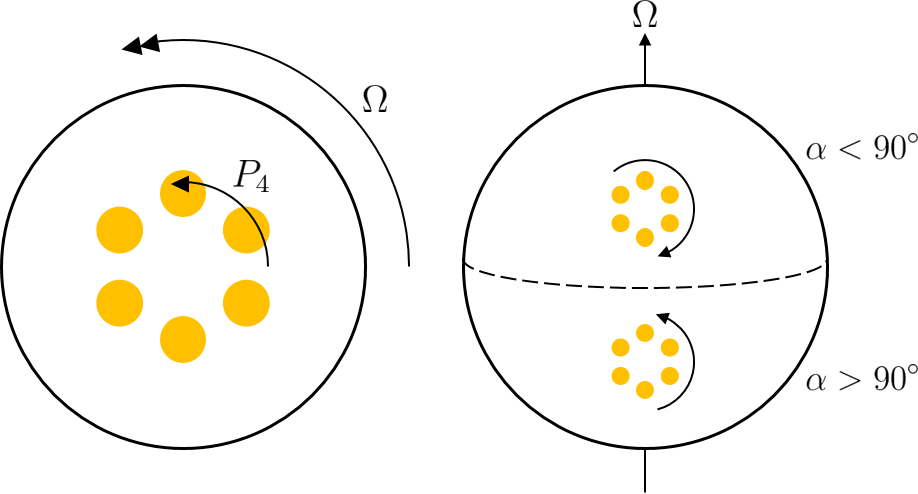
\includegraphics[width=0.75\textwidth]{Figures/geometry_appendix/carousel_direction}
        \caption[Circulation direction of the carousel]{A carousel-like structure in the polar emission region circulates in the same direction as the pulsar rotates, but slower \citep{RSxx1975}. The left-hand panel illustrates this for an aligned rotator ($\alpha = 0$). The result is that to an observer corotating with the star the carousel rotates clockwise about the magnetic axis in the northern hemisphere ($\alpha < 90\degr$), and anticlockwise in the southern hemisphere ($\alpha > 90\degr$) as illustrated in the right-hand panel.}
        \label{fig: geometry derivations - carousel direction}
    \end{center}
\end{figure}
When creating a beam map, it is necessary to do some form of interpolation to map the observed emission which is only visible once per rotation to a rectangular grid of points in the beam map -- the method used in this work is bilinear interpolation.

Care needs to be taken to avoid confusion with signs. Both $P_4$ and $P_3$ I define as positive quantities, as they are time periods. $\Theta$ is defined such that it is increasing in a clockwise direction as seen by the observer if $\alpha$ is defined with respect to the angular momentum vector $\mathbf{\Omega}$. This implies that if $\alpha$ is derived from the RVM, care must be taken in defining the direction of the PA consistently \citep[see][]{EWxx2001}. At $\phi = \phi_\mathrm{fid}$ for $k = 0$, emission directed at an angle of $\Theta = 0$ is observed.

The total azimuthal offset $\Theta$ is simply the sum of $\theta_\mathrm{trans}$ and $\theta_\mathrm{rot}$,
\begin{equation}
	\Theta = \theta_\mathrm{trans}+\theta_\mathrm{rot}.
    \label{eq: geometry derivations - derived Theta}
\end{equation}






\subsubsection{The reverse transformation and contours of constant \texorpdfstring{$\Theta$}{Theta}}
\label{app: geometry derivations - cartographic transforms - reverse transformation}

Equations \eqref{eq: cartographic transform - R}$-$\eqref{eq: cartographic transform - theta_rot} define the transform to go from the pulse stack ($\phi$, $k$) to the carousel frame ($R$, $\Theta$). It is useful to explicitly state the reverse transform. The pulse longitude $\phi$ can be found directly by inverting Eq.~\eqref{eq: cartographic transform - R} -- note that a given $R$ corresponds to two points on opposite sides of and equidistant to $\phi_\mathrm{fid}$. Equation~\eqref{eq: thetarot} can be substituted into Eq~\eqref{eq: geometry derivations - derived Theta} which can then be simply rearranged to calculate the pulse number $k$ as a function of pulse longitude $\phi$,
\begin{equation}
    \label{eq: geometry derivations - raw k as function of phi}
    k(\phi) = -\frac{\phi - \phi_\mathrm{fid}}{2\pi} \mp \frac{P_4}{2\pi P_1}\big(\Theta - \theta_\mathrm{trans}(\phi) \big),
\end{equation}
where $\theta_\mathrm{trans}$ is explicitly expressed as a function of $\phi$. This can be considered to be a `contour of constant $\Theta$', and closely represents what the expected driftband shape should be if the sub-beams are compact.


















\section{Extension of the cartographic transform to aliasing}
\label{app: geometry derivations - aliasing}

For slowly rotating carousels, the observed modulation period $P_3$ is equivalent to the time it takes for a sub-beam in the carousel to drift round to the position of its neighbour. As discussed in detail by for example \citet{GGKS2004}, in the case of fast drift the measured repetition period of the subpulse pattern $P_3$ can be larger than the true time $P_3^t \equiv P_4/N$ it takes for the carousel to drift by one sub-beam separation. This is due to aliasing, the consequence of the drift pattern being sampled once per rotation period $P_1$ of the star, which occurs when $P_3^t < 2P_1$. The relation between the observed and actual drift of the carousel depends on the alias order $n$ (here defined as a nonnegative integer) such that for odd $n$ the apparent drift direction is opposite to the true drift direction. The apparent $P_3$ is related to the actual circulation period of the carousel via
\begin{equation}
    \label{eq: geometry derivations - aliasing equation P3}
    \frac{s}{P_1} + \frac{(-1)^n}{P_3} = \frac{1}{P_3^t} = \frac{N}{P_4},
\end{equation}
where $s = \text{int}[(n+1)/2]$ (here `int' is the function which returns the integer part of its argument). I define all variables in Eq.~\eqref{eq: geometry derivations - aliasing equation P3} to be positive since the carousel drift direction is described by the sign modifier discussed in Appendix~\ref{app: geometry derivations - cartographic transforms - derivation of Theta - theta rot}. This sign modifier is defined in terms of the actual drift direction rather than the perceived drift direction. The cartographic transform equations and contour of constant $\Theta$ remain valid in the case of aliasing, except that $P_4$ must now be related to the observed $P_3$, $N$, and $n$ via Eq.~\eqref{eq: geometry derivations - aliasing equation P3}. 





























\section{The cartographic transform applied to folded data}
\label{app: geometry derivations - P3 fold}

% Equation~\eqref{eq: geometry derivations - raw k as function of phi} defines a contour of constant carousel azimuth $\Theta$ in a pulse stack, defined by pulse longitude $\phi$ and pulse number $k$. If the carousel is circulating fast enough such that aliasing effects are present, the circulation period $P_4$ is related to the observed modulation period $P_3$ according to Eq.~\eqref{eq: geometry derivations - aliasing equation P3}. What if the data has now been folded at $P_3$? How then is Eq.~\eqref{eq: geometry derivations - raw k as function of phi} modified to define the driftbands seen in a $P_3$-fold? 

In a $P_3$-fold, the pulse number $k$ is cyclically related to a phase in the modulation cycle, $\Phi = [0, 2\pi]$. The transformation from coordinates ($R$, $\Theta$) in the carousel frame to $k$ and $\phi$ is explained in Sec.~\ref{app: geometry derivations - cartographic transforms - reverse transformation}, and a given pulse number can be expressed as a $P_3$ phase, which will be cyclic over a period of $P_4/N$. This period can be less than $2P_1$ if aliasing is occurring.  Folding effectively averages out any differences in sub-beam morphology, so the beamlets resulting from this mapped cartographic transform will be identical. To map $\Phi$ to a phase in the $P_3$ cycle, a factor of $(-1)^n$ is needed to take into account any apparent drift direction change associated with different alias orders, $n$. In summary, 
\begin{equation}
    \label{eq: geometry derivations - P3 phase definition}
    % \Phi = \frac{N}{P_4} \cdot (-1)^n P_3 \cdot k.
    \Phi = 2\pi(-1)^n\cdot \frac{NP_1}{P_4} \cdot k,
\end{equation}
where $k$ is calculated from Eq.~\eqref{eq: geometry derivations - raw k as function of phi}.
%Strictly speaking Eq.~\eqref{eq: geometry derivations - P3 phase definition} is modulo $P_3$ to map a given carousel coordinate ($R$, $\Theta$) to within the cycle. 






\subsection{Expected driftband shape in folded data}
\label{app: geometry derivations - P3 fold - driftband shape}

Equation~\eqref{eq: geometry derivations - raw k as function of phi} can be used to define a contour of constant carousel azimuth $\Theta$ in a pulse stack, defined by pulse longitude $\phi$ and pulse number $k$. What if the data has now been folded at $P_3$? How then is Eq.~\eqref{eq: geometry derivations - raw k as function of phi} modified to define the driftbands seen in a $P_3$-fold? The theoretical driftband gradient for a given carousel structure can be calculated from Eq.~\eqref{eq: geometry derivations - P3 phase definition} by differentiating with respect to $\phi$. This is
\begin{equation}
    \label{eq: geometry derivations - derivative of P3 phase}
    % \dphi{\Phi} = \frac{(-1)^n N P_3}{P_4}  \cdot \dphi{k},
    \dphi{\Phi} = 2\pi(-1)^n\cdot \frac{NP_1}{P_4} \cdot \dphi{k},
\end{equation}
where (using Eq.~\eqref{eq: geometry derivations - raw k as function of phi} with constant $\Theta$)
\begin{equation}
    \dphi{k} = -\frac{1}{2\pi}\pm\frac{P_4}{2\pi P_1}\dphi{\theta_\mathrm{trans}}.
    \label{eq: geometry derivations - derivative of k}
\end{equation}
The differential of $\theta_\mathrm{trans}$ can be calculated from Eq.~\eqref{eq: cartographic transform - sin theta_trans}. Let $\theta_\mathrm{trans} = \arcsin{x}$, where $x$ is the right-hand side of Eq.~\eqref{eq: cartographic transform - sin theta_trans}. Then, 
\begin{equation}
    \label{eq: geometry derivations - derivative of ttrans full}
    \dphi{\theta_\mathrm{trans}} = \frac{1}{\sqrt{1-x^2}} \bigg[\frac{\sin(\alpha + \beta) \cos(\phi-\phi_\mathrm{fid})}{\sin R} - \frac{\sin(\alpha + \beta) \sin(\phi-\phi_\mathrm{fid})}{\sin^2 R} \dphi{\sin R}\bigg].
\end{equation}
For a driftband which only occupies a narrow longitude range around (what is presumed to be) the fiducial plane, we are interested in the gradient near $\phi = \phi_\mathrm{fid}$. Here, $R=\beta$ and $\theta_\mathrm{trans}= x = 0$, so Eq.~\eqref{eq: geometry derivations - derivative of ttrans full} reduces to
\begin{equation}
    \label{eq: geometry derivations - derivative of ttrans phifid}
    \dphi{\theta_\mathrm{trans}}\bigg|_{\phi_\mathrm{fid}} = \frac{\sin(\alpha + \beta)}{\sin\beta},
\end{equation}
which is incidentally very similar to the gradient of the Rotating Vector Model at its inflection point, $\sin\alpha / \sin\beta$ (Sec.~\ref{sec: intro - emission models - polarisation - RVM}). This can be substituted back into Eqs.~\eqref{eq: geometry derivations - derivative of P3 phase} and \eqref{eq: geometry derivations - derivative of k} to give the expected gradient $m$ of the driftband in the $P_3$-fold,
\begin{equation}
    \label{eq: driftband gradient}
    % m = \dphi{\Phi}\bigg|_{\phi_\mathrm{fid}} = -\frac{(-1)^nNP_3}{2\pi}\bigg(\frac{1}{P_4} \mp \frac{1}{P_1}\frac{\sin(\alpha + \beta)}{\sin\beta}\bigg).
    m = \dphi{\Phi}\bigg|_{\phi_\mathrm{fid}} = N(-1)^{n+1} \bigg(\frac{P_1}{P_4} \mp \frac{\sin(\alpha + \beta)}{\sin\beta}\bigg)
\end{equation}
When a grid search over pulsar geometry parameters is performed as in Chapter~\ref{chapt: B0031}, it can be desirable to define the grid in terms of $m$ in order to avoid the exploration of parameters that produce solutions with driftband gradients that do not resemble the observations. In examining the two drift modes of PSR~B0031$-$07, $m$ was used as a proxy for the line-of-sight impact parameter $\beta$. This can subsequently be found from a given choice of $\alpha$, $N$, $n$, and $m$ by rearranging Eq.~\eqref{eq: driftband gradient} to give
\begin{equation}
    \label{eq: geometry derivations - beta from gradient}
    \beta = \arctan\bigg(\frac{\sin\alpha}{Q - \cos\alpha}\bigg),
\end{equation}
where 
\begin{equation}
    \label{eq: geometry derivations - definition of Q}
    Q = \pm \bigg(\frac{P_1}{P_4} + (-1)^n\frac{m}{N} \bigg).
\end{equation}
The convention of the $\pm$ sign is the same as defined earlier: the upper sign ($+$ in this case) corresponds to geometries with $\alpha < 90\degr$, whilst the lower sign ($-$) corresponds to $\alpha > 90\degr$.

Care needs to be taken to ensure that $m$ as defined in Eq.~\eqref{eq: driftband gradient} is a dimensionless number. When measured in units of pulse numbers per radian (as was done in Chapter~\ref{chapt: B0031}), it first needs to be multiplied by $2\pi P_1/P_3$ to make it dimensionless. Likewise, if measured in units of pulse numbers per degree it should be multiplied first by $360P_1/P_3$ before applying Eq.~\eqref{eq: geometry derivations - definition of Q}.






\subsection{Finding pairs of matching points}
\label{app: geometry derivations - P3 fold - matching points}

Since the cartographic transform is periodic, the emission from a given set of coordinates ($R$, $\Theta$) is observable at different times as parametrised by coordinates in the pulse stack or $P_3$-fold ($\phi$, $k$). Particularly relevant here is that coordinates ($R$, $\Theta$) map to two different pulse longitudes $\phi_1$ and $\phi_2$ which are related such that
\begin{equation}
    \label{eq: geometry derivations - opposite phi}
    \phi_2 = 2\phi_\mathrm{fid} - \phi_1,
\end{equation}
i.e. the fiducial plane lies exactly in between these longitudes. The LOS can intersect the same point in the carousel at longitudes $\phi_1$ and $\phi_2$ at different pulse numbers $k_1$ and $k_2$ such that
\begin{equation}
    \label{eq: geometry derivations - opposite k}
    k_2 = k_1 + \Delta k + n_\mathrm{arb}\frac{P_4}{P_1},
\end{equation}
where
\begin{equation}
    \label{eq: delta k stack}
    \Delta k = \frac{1}{2\pi}\bigg[\phi_1 - \phi_2 \pm \frac{P_4}{P_1}\Big(\theta_\mathrm{trans}(\phi_2) - \theta_\mathrm{trans}(\phi_1)\Big)\bigg].
\end{equation}
and $n_\mathrm{arb}$ is an arbitrary integer. In the sign convention followed, $+$ corresponds to $\alpha<90\degr$ and $-$ for $\alpha > 90\degr$. Note that only if $k_2 - k_1$ is an integer the exact same point $(R,\ \Theta)$ in the carousel is \textit{exactly} observable at two different times. When $P_3$-folds are considered, this becomes
\begin{equation}
    \label{eq: P3 fold phase}
    % \Phi_2 = \bigg(\Phi_1 + (-1)^n\frac{ N P_3}{P4}\Delta k \bigg)\mod{\frac{P_3}{P_1}}
    \Phi_2 = \Phi_1 + 2\pi(-1)^n\frac{ N P_1}{P_4}\Delta k
\end{equation}

Under the assumption that the sub-beam pattern is static apart from its circulation, the corresponding pairs of points in the $P_3$-fold are expected to have identical emission properties, although the position angle could have rotated, possibly following the prediction of the RVM. In Chapter~\ref{chapt: B0031} these effects are however removed from the data in the process of separating the OPMs, as described in Sec.~\ref{sec: B0031 - methods - mode separation}.

